\documentclass{article}

\usepackage[ngerman]{babel}
\usepackage[utf8]{inputenc}
\usepackage[T1]{fontenc}
\usepackage{hyperref}
\usepackage{csq uotes}
\usepackage[a4paper]{geometry}
\usepackage{graphicx}
\usepackage{float}
\usepackage{caption}

\usepackage[
    backend=biber,
    style=apa,
    sortlocale=de_DE,
    natbib=true,
    url=false,
    doi=false,
    sortcites=true,
    sorting=nyt,
    isbn=false,
    hyperref=true,
    backref=false,
    giveninits=false,
    eprint=false]{biblatex}
\addbibresource{../references/bibliography.bib}


\title{Ethik im Umgang mit Daten}
\author{Jaël Theiler}
\date{31.05.24}


\begin{document}

\maketitle

\abstract{
    Künstliche Intelligenz (KI) ermöglicht es Computern, Aufgaben zu erledigen, die normalerweise menschliche Intelligenz erfordern. Zum Beispiel Lernen, Problemlösen und Sprachverstehen. Im Alltag begegnen wir der KI zum Beispiel in Sprachassistenten wie Siri und Alexa, Empfehlungssysteme auf Plattformen wie Netflix und Amazon sowie bei den selbstfahrende Autos.
    Um die KI zu trainieren wird z.B. das maschinelle Lernen (ML) angewendet, bei dem der Computer aus grossen Datenmengen Muster erkennt und analysiert. Neuronale Netze, die dem menschlichen Gehirn nachempfinden, spielen dabei eine wichtige Rolle. Das Neuronale Netz ist ein Modell, welches mit Prozessen nachahmen soll wie biologische Neuronen zusammenarbeiten um möglichst Entscheidungen so zu treffen wie das menschliche Gehirn es tun würde. So versucht die KI möglichst verständliche Schlussfolgerungen zuziehen und seine Antworten zu optimieren.
    
}

\tableofcontents

\section{Künstliche Intelligenz}
\subsection{Was sind Künstliche Intelligenz?}
Wie der Name bereits sagt, ist die Künstliche Intelligenz (KI) ein Versuch die menschliche Intelligenz zu rekreieren. Sie ermöglicht es Computern, Aufgaben zu erledigen, die normalerweise menschliche Intelligenz erfordern. Zum Beispiel Lernen, Problemlösen und Sprachverstehen. Im Alltag begegnen wir der KI zum Beispiel in Sprachassistenten wie Siri und Alexa, Empfehlungssysteme auf Plattformen wie Netflix und Amazon sowie bei den selbstfahrende Autos.
Um die KI zu trainieren wird z.B. das maschinelle Lernen (ML) angewendet, bei dem der Computer aus grossen Datenmengen Muster erkennt und analysiert. Neuronale Netze, die dem menschlichen Gehirn nachempfinden, spielen dabei eine wichtige Rolle. Das Neuronale Netz ist ein Modell, welches mit Prozessen nachahmen soll wie biologische Neuronen zusammenarbeiten um möglichst Entscheidungen so zu treffen wie das menschliche Gehirn es tun würde. So versucht die KI möglichst verständliche Schlussfolgerungen zuziehen und seine Antworten zu optimieren.

\subsection{Wie wird KI trainiert?}

\section{Cookies}

\subsection{Was sind Cookies?}
Cookies sind einfach gesagt Textdateien, die bei einem Besuch einer Webseite von einem Server auf das Gerät des Users übertragen werden. Diese Dateien enthalten Informationen, die es der Webseite ermöglichen, den Nutzer bei zukünftigen Besuchen wiederzuerkennen und bestimmte Einstellungen oder Präferenzen beizubehalten. Diese Textdateien bleiben auch auf diesem Gerät bis sie entweder gelöscht werden, ihr Verfallsdatum erreichen oder man die Website wieder besucht, denn dann werden sie wieder auf den Server übertragen. Die Verfallsdaten, können  von der Schliessung der Website bis mehrere Jahre nach dem Besuch dauern.Die Dauer hängt von dem Zweck der Cookies ab. Cookies spielen eine wichtige Rolle im modernen Web, da es Webseiten ermöglichen, effizienter zu arbeiten. Sie werden unter anderem für Funktionen wie die Benutzeranmeldung, die Personalisierung von Inhalten und die Analyse des Nutzerverhaltens verwendet. Viele Unternehmen nutzen Cookies wegen diesen und noch ein paar anderen Gründen.

\subsection{Arten von Cookies}
Zusätzlich zu den standart Funktionen von Cookies gibt es noch verschiedene Arten davon, welche andere Aufgaben und Zwecke erfüllen. Dafür kann man sie zuerst in zwei Untergruppen teilen; den technisch notwendigen Cookies und den technisch nicht notwendigen Cookies. 
Technisch notwendige Cookies sind zum Beispiel Session Cookies. Sie speichern deine User Einstellungen wie auch Spracheinstellungen. Paypal ist beispielsweise ein Nutzer von Session Cookies. Wenn du dich bei deinem PayPal-Konto anmeldest, setzt PayPal ein Cookie auf dein Gerät, um dich während deiner Browsersitzung angemeldet zu halten. Dadurch musst du dich nicht bei jeder Transaktion erneut anmelden.
Diese Cookies werden auch verwendet, um die Sicherheit deines PayPal-Kontos zu gewährleisten. Sie können auch dazu beitragen, betrügerische Aktivitäten zu erkennen, indem sie Informationen über deine früheren Transaktionen und Anmeldeaktivitäten speichern und analysieren. Diese Art von Cookies dienen alleine zur Funktionsfähigkeit und Sicherheit einer Webseite.
Die technisch nicht notwendigen Cookies werden eher aus anderen Gründen genutzt. Sie dienen oft dazu, zusätzliche Funktionen zu ermöglichen oder das Nutzererlebnis zu verbessern. Jedoch sind sie nicht essenziell für Kernfunktionen einer Webseite. Beispiele für diese Cookies sind Marketing-,Analyse-, Statistik-, Personalisierungs- und Social Media- Cookies. Die Marketing Cookies verfolgen das Verhalten der Nutzer um personalisierte Werbung anzuzeigen. Andere sind dazu da den Betreibern dieser Webseiten zu helfen die Popularität ihrer Inhalte zu verstehen und auch die Anzahl der Nutzer zu messen. Jedoch müssen diese nicht notwendigen Cookies ausdrücklich von den Nutzer bewilligt werden. Das geschieht in der Regel durch eine Banner-Nachricht die oftmals beim ersten Besuch der Webseite angezeigt wird. Dort hat man dann die Wahl die Cookies zu akzeptieren oder die Cookieeinstellungen zu ändern.


 
\begin{figure}[ht]
    \centering
    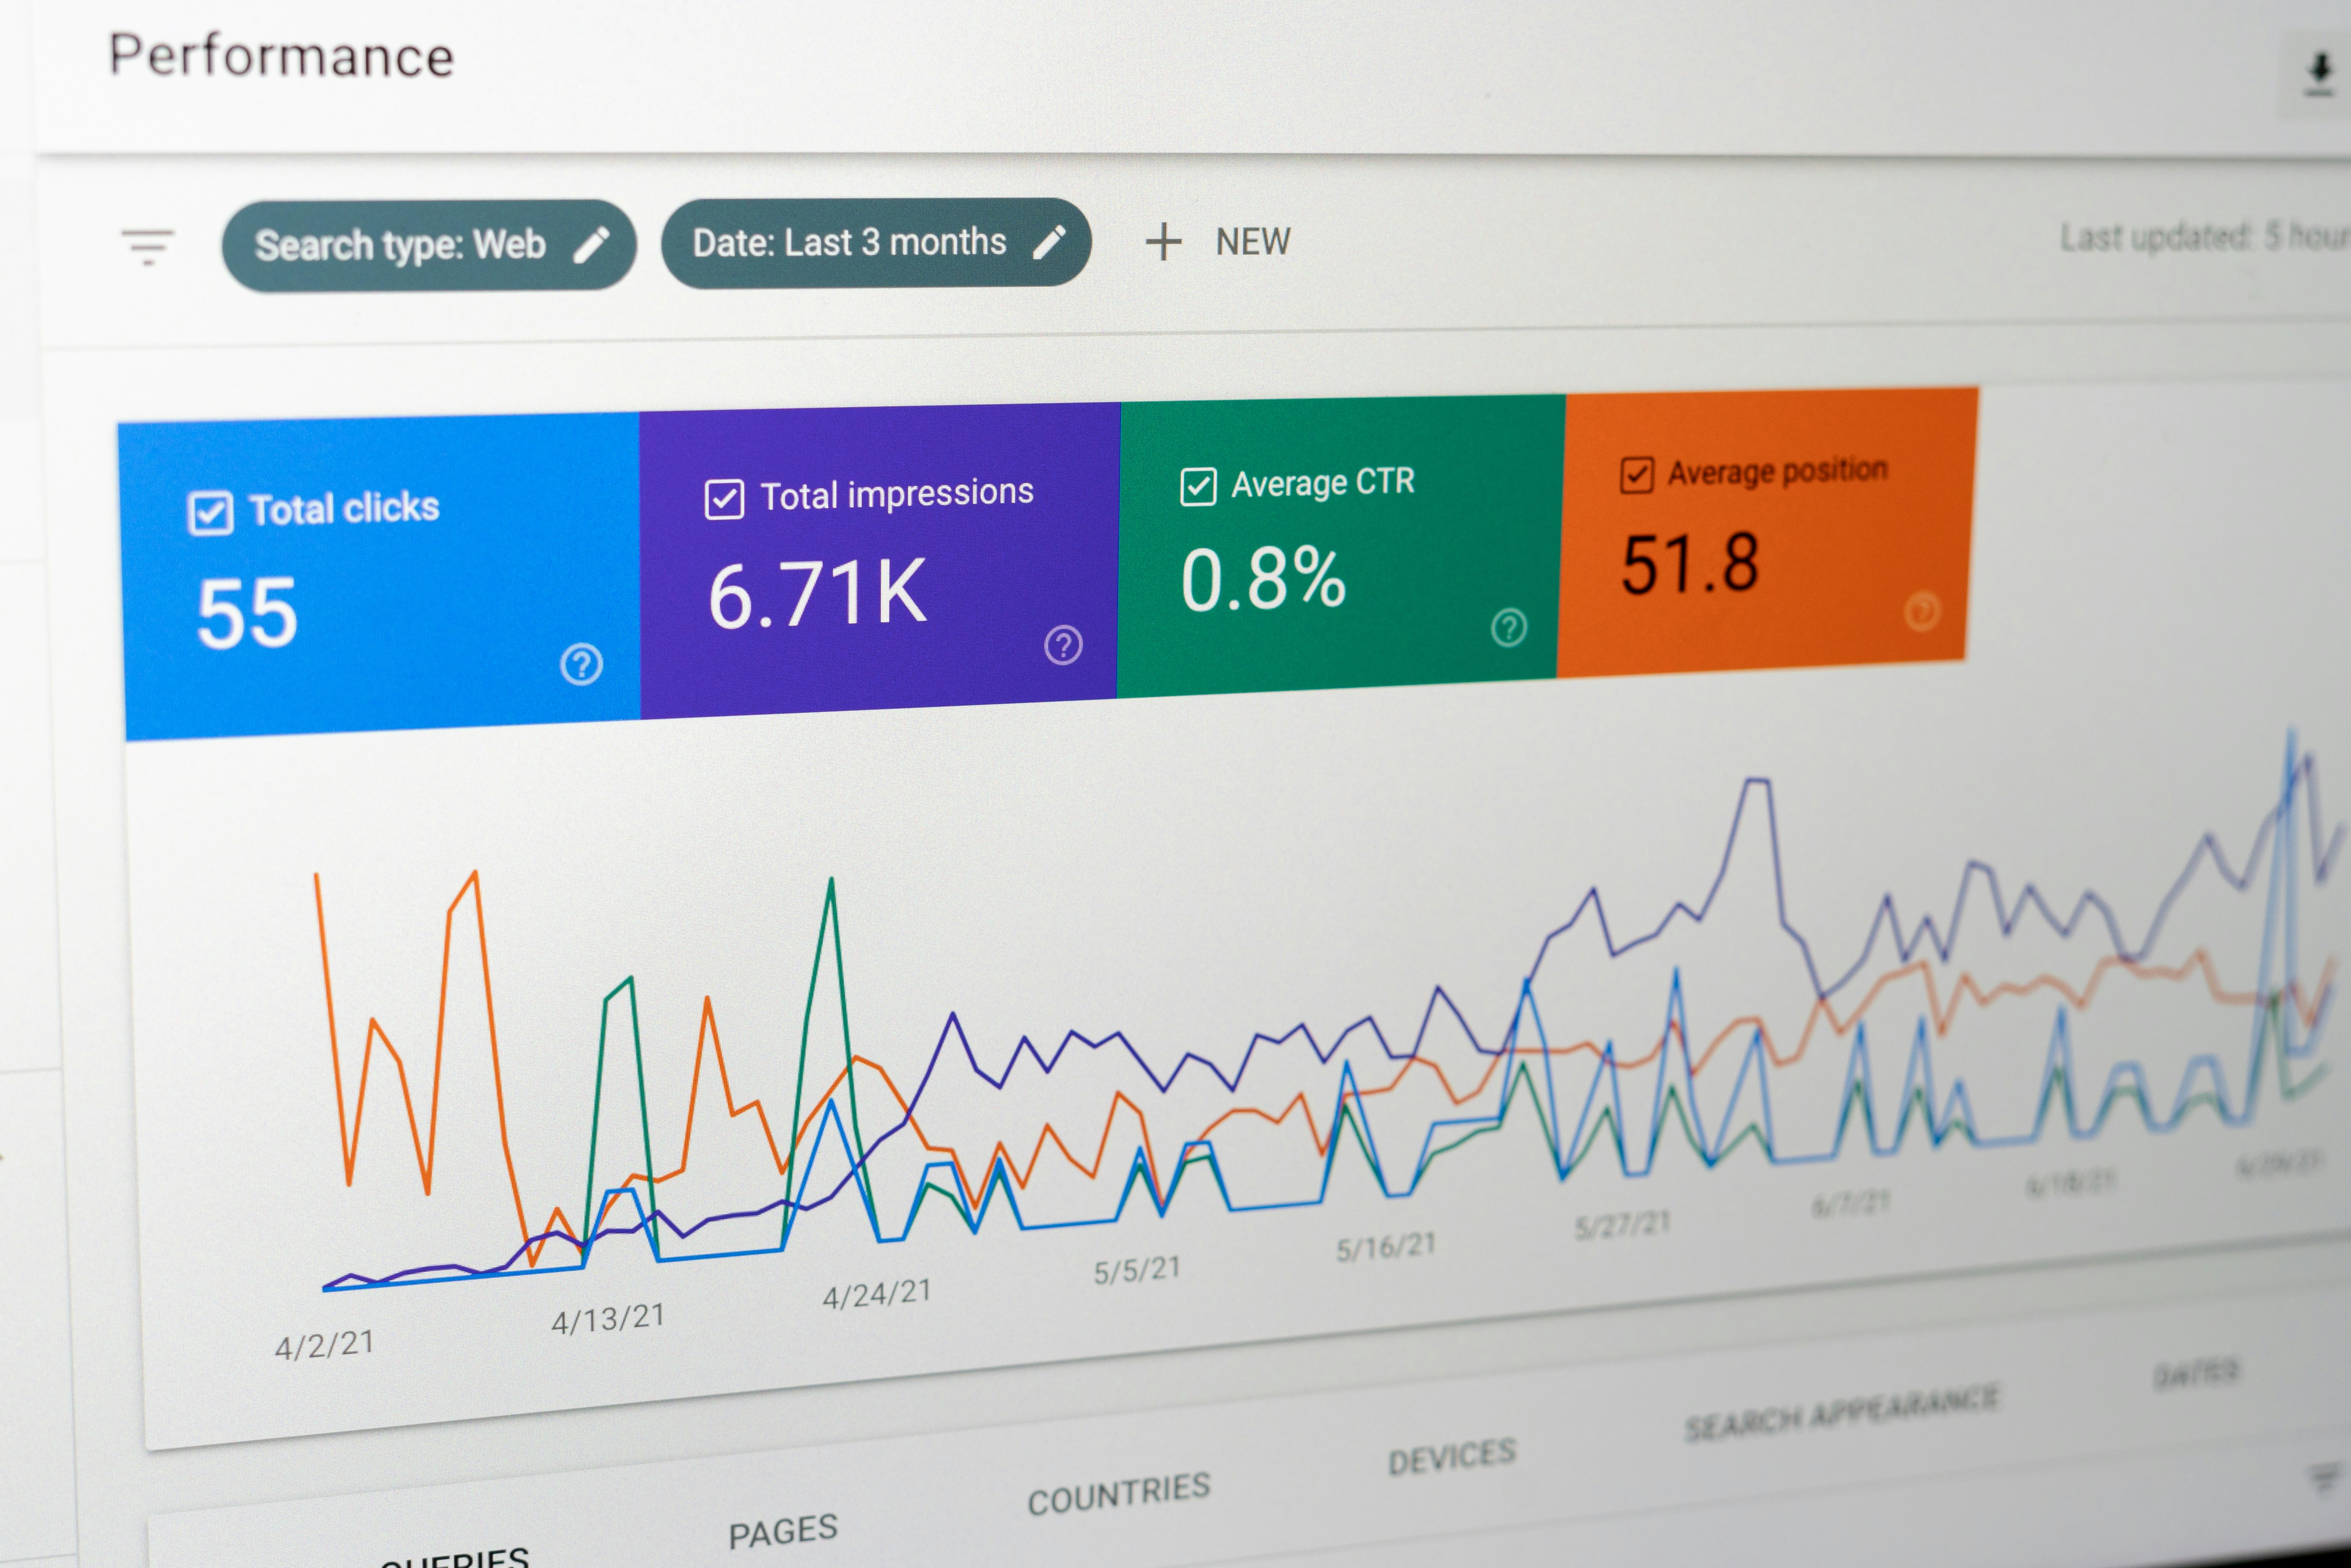
\includegraphics[width=0.6\textwidth]{Statistik.jpg}
    \caption{Statistik}
    \label{fig:Statistik}
    \end{figure}
 

\subsection{Datenschutz der Cookies}
Die Verwendung dieser Cookies ist in der EU durch die Datenschutz-Grundverordnung (DSGVO) und die ePrivacy-Richtlinie geregelt. Nutzer müssen klar und umfassend über die Verwendung dieser Cookies informiert werden und die Möglichkeit haben, ihre Einwilligung zu geben oder abzulehnen. Viele Websites informieren jedoch die Nutzer nicht ausreichend über die Art der gesammelten Daten und die Zwecke der Datenverarbeitung oder die Datenschutzrichtlinien sind oft lang und sehr kompliziert, weshalb viele Nutzer die genauen Implikationen der Cookie-Nutzung nicht verstehen und so keine realistische Entscheidung treffen können.
Technisch nicht notwendige Cookies werden auch oft verwendet, um das Verhalten der Nutzer über verschiedene Websites hinweg zu verfolgen, zum Beispiel durc Analyse-dienste. Dies führt zu umfangreichen Profilen, die detaillierte Informationen über das Online-Verhalten und die Vorlieben der Nutzer enthalten.Diese Informationen können dann beispielsweise für Personalisierte Werbung genutzt werden, was auf einer Seite einen Vorteil für die Nutzer sein kann aber auf der anderen Seite eine Gefahr für die Privatsphäre der Nutzer darstellt.
Viele der technisch nicht notwendige Cookies stammen zusätzlich auch von Drittanbietern(z.B Analyse-Dienste). Die Weitergabe von Daten an diese Drittanbieter kann zu Datenschutzproblemen führen, insbesondere wenn die Drittanbieter in Ländern mit weniger strengen Datenschutzgesetzen sind.Nutzer haben oft wenig bis gar keine Kontrolle darüber, welche Drittanbieter Zugang zu ihren Daten haben und wie diese Daten verwendet werden.Nutzer haben oft wenig bis gar keine Kontrolle darüber, welche Drittanbieter Zugang zu ihren Daten haben und wie diese Daten verwendet werden. Die Problematik liegt auch darin, dass die Nutzer haben dabei oft wenig bis gar keine Kontrolle darüber, welche Drittanbieter Zugang zu ihren Daten haben und wie diese Daten verwendet werden. 

\nocite{*}
\printbibliography

\end{document}
